%Heat Capacity Error
%SS

\section{Error in Specific Heat Calculation}\label{errorinspecificheatcalculation}

Error in this part of the experiment predominantly arises due to the statistical error in the calibration of the germanium resistor.  Although the fitting parameters shown in Eqn. \ref{eq:polyfit} yield an $r^{2}$-value of greater than $0.999$, the error in those parameters reduced the level of precision with which we could determine temperature.  

To determine the relative error attributed to each temperature value we noted that the error was comprised of the error in the measured electric potential across the germanium resistor and error in the nine fitting parameters.  The relative error in the electric potential across the resistor was noted to be roughly $1\%$.  The error in the fitting parameters was given by the nonlinear regression analysis.  Adding the relative errors in quadrature, we determine that the relative error in temperature, $\Delta T/T$ is a function of temperature, as in Fig. \ref{fig:temperror}.  

\begin{figure}[htbp]
\begin{center}
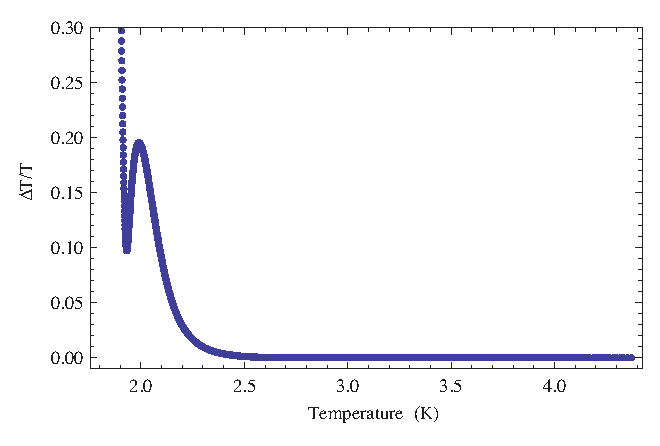
\includegraphics[height=70mm]{./figures/temperror.eps}
\caption{\small{The relationship between relative error in temperature and the temperature of the cell.}}
\label{fig:temperror}
\end{center}
\end{figure}

With this calculation we can calculate the relative error in the temperature at the value corresponding to $V_{\lambda}$ determined in Section \ref{calculatingtheheatcapacityofthecell}.  This relative error must be added in quadrature with the relative uncertainty in $V_{\lambda}$, namely $0.16\%$ (corresponding to a $2$ mV interval at $671$ mV).  This uncertainty is different from measurement error: this is the interval over which $V_{\lambda}$ could occur based on our interpretation of the data in Fig. \ref{fig:rawdata} (b).  This error in the uncertainty of $V_{\lambda}$ is so small, however, that it doesn't add to the relative error in temperature shown in Fig. \ref{fig:temperror}.  Ultimately, we find that for our measured value of $T_{\lambda}$ there is an error of $3.7\%$.  Therefore, our measurement of $T_{\lambda}$ is $2.178\pm0.081 K$.

To calculate the relative error in specific heat, we decompose the expression 

\begin{center}
\begin{equation}
C_{sat}=\frac{V_{R}^{2}}{\Delta T R_{R}}\Delta t_{pulse} \frac{R_{ideal}T_{room}}{P_{gas}V_{gas}}
\end{equation}
\end{center}

where $C_{sat}$ is the specific heat of He, $V_{R}$ and $R_{R}$ are the electric potential and the resistance of the heater, $\Delta T$ is the resulting change in temperature due to a heat pulse, $\Delta t_{pulse}$ is the length of the heat pulse, $R_{ideal}$ is the ideal gas constant, $T_{room}$ is room temperature, $P_{gas}$ is the pressure of some volume $V_{gas}$ of He.  From this equation and the relative measurement errors of each of the variables, we can determine the the relative error in specific heat as a function of temperature.  Without factoring in the error in temperature which we previously described, we find that each specific heat value is at a constant value of $14\%$ for all temperatures.  To add the effect of the error in temperature we add the these two values in quadrature.  Finally, because our final specific heat data is averaged by $N=3$, we must divide this error by $\sqrt{3-1}$. As expected our final error in specific heat varies with temperature as shown in Fig. \ref{fig:heatcaperror}.

\begin{figure}[htbp]
\begin{center}
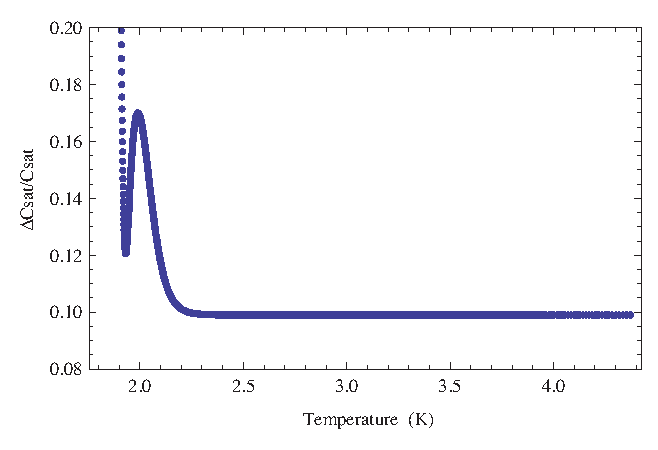
\includegraphics[height=70mm]{./figures/heatcaperror.eps}
\caption{\small{The relationship between relative error in specific heat and temperature of helium.}}
\label{fig:heatcaperror}
\end{center}
\end{figure}

Note that the error in specific heat ranges from $10\%$ to $17\%$.  This error is minimal compared to the overall range in specific heats observed and explains some of the variation in data shown in Fig. \ref{fig:lambdatrans}.